\documentclass[a4paper,utf8]{article}
\usepackage[heading,fancyhdr]{ctex}
\usepackage{amsmath,amssymb,geometry,lastpage,ulem}
\usepackage{array,tabularx,tabulary,mhchem,xspace}
\usepackage{floatrow,subfig,multirow,bigstrut}
\usepackage{siunitx,booktabs,longtable,graphicx,xfrac,nameref}
\lineskiplimit=1pt
\lineskip=3pt
\geometry{
    top=25.4mm, 
    left=25mm, 
    right=25mm, 
    bottom=25mm,
    headsep=5.9mm,
}
\ctexset{
    section = {format+=\raggedright}
}
\newcommand{\fgref}[1]{图~\ref{#1}\xspace}
\newcommand{\seqref}[1]{式~(\ref{#1})}
\newcommand{\expinfo}[7][无]{
    {\zihao{-3}\bfseries\songti
    实验名称:\uline{\hfill\mbox{#2}\hfill} \\[2.9mm]
    学\quad 号:\uline{\makebox[25mm]{#3}}\hfill
    姓\quad 名:\uline{\makebox[25mm]{#4}}\hfill
    班\quad 级:\uline{\makebox[25mm]{#5}} \\[2.9mm]
    合作者:\uline{\makebox[25mm]{#1}} \hfill
    桌\quad 号:\uline{\makebox[25mm]{#6}}\hfill\makebox[25mm+4em]{}\\[2.9mm]
    实验日期:\uline{\makebox[30mm]{#7}}\hfill\mbox{} \\[58.7mm]
    }
}
\newcommand{\pointingbox}{
    {\zihao{4}\bfseries\songti%
    实验考核\\[3mm]
    \extrarowheight=3mm
    \begin{tabularx}{150mm}{|X|X|X|X|X|}\hline
        \hfil 项目 \hfil  & \hfil 实验预习 \hfil & \hfil 实验过程 \hfil & \hfil 分析与讨论 \hfil & \hfil 总评 \hfil \\[3mm] \hline
        \hfil 评价 \hfil &  &  &  &  \\[3mm] \hline
    \end{tabularx}
    }
}
\newcommand{\derivative}[2]{\frac{\mathrm{d} #1}{\mathrm{d} #2}}
\newcommand{\thinking}[2]{\textbf{#1}\\
答:\begin{minipage}[t]{0.85\textwidth}
    #2
\end{minipage}}
\pagestyle{fancy}
\fancyhf{} \fancyhead[C]{电路基础实验} \fancyfoot[C]{\thepage~/~\pageref{LastPage}}
\newcounter{Rownumber}
\newcommand*{\Rown}{\stepcounter{Rownumber}\theRownumber}
\newcommand*{\resetRown}{\setcounter{Rownumber}{0}}
\newcommand{\qrange}[3]{\qtyrange[range-phrase = \text{$\sim$},range-units =single]{#1}{#2}{#3}}
\floatsetup[table]{capposition=top}
\newcolumntype{C}{>{\hfil}X<{\hfil}}
\renewcommand{\Nameref}[1]{\textbf{\ref{#1}~\nameref{#1}}} %导入导言
\begin{document}
\begin{center}
    {\mbox{}\\[7em]\zihao{2}\bfseries\songti%
    电路基础实验报告}\\[34mm]
    \expinfo[王慷]{仪器入门及电位、电压的测量}{22301056}{王俊杰}{22 材物}{27}{2024.4.30}
\end{center}
\newpage
\section{实验目的}
\begin{enumerate}
    \item 了解万用表和直流稳压电源的基本功能并掌握其使用方法
    \item 了解电路分析实验箱的基本构造并掌握其使用方法
    \item 用实验证明电路中电位的相对性和电压的绝对性
\end{enumerate}

\section{实验原理及电路图}%简单描述,含必要的公式和附图;
    \subsection{实验原理}
    \subsubsection{万用表}
        万用表是用于测量电路的各种基本电参数的设备,可以测量交直流电压、电流、电阻阻值、电容值和二极管等。万用表的主要技术指标是测量精度,通常有 3\sfrac{1}{2},4\sfrac{1}{2},5\sfrac{1}{2},6\sfrac{1}{2}位等不同规格,以 5\sfrac{1}{2} 位的万用表为例,它可以显示 6 位数字,第一位数字只能显示 0 或 1,也就是半位,后面可以显示 5 位数字。测量显示的位数越多,说明仪表的分辨率越高,精度也越高。实验所用的万用表为 RIGOL DM3058 万用表。\par
        使用方法:
        \begin{enumerate}
            \item 选择功能
            \item 选择量程,量程的选择有自动和手动两种方式。实验室使用的万用表可以根据输入信号自动选择合适的量程, 这对用户来说是非常方便的,开机后默认是自动量程。
            \item 与被测元件连接,进行测量。测量电流时,万用表要与被测元件串联,测量电压、电阻、电容、二极管等时,万用表要与被测元件并联
        \end{enumerate}

    \subsubsection{直流稳压电源}
        实验室使用的是 RIGOL DP832 直流稳压电源,提供三种输出模式:恒压输出(CV)、恒流输出(CC)和临界模式(UR)。在 CV 模式下,输出电压等于电压设置值,输出电流由负载决定;在 CC 模式下,输出电流等于电流设置值,输出电压由负载决定;UR 是介于 CV 和 CC 之间的临界模式。\par
        使用方法:
        \begin{enumerate}
            \item 选择要设置的通道
            \item 设置输出电压、电流
            \item 设置过压过流保护
            \item 打开输出
        \end{enumerate}
        
    \subsubsection{电路中电位与电压的测量}
        一个确定的闭合电路中,各点电位的高低视所选电位参考点的不同而变,但任意两点间的电位差(即电压)是绝对的,它不因参考点的变动而改变。据此性质,我们可以用电压表来测量出电路中各点的电位及任意两点间的电压。\par
        以电路中的电位值为纵坐标,电路中各点位置为横坐标,将测量到的各点电位在该坐标平面中标出,并把标出的点按顺序用直线相连接,就可得到电路的电位变化图。每一段直线段即表示两点间电位的变化情况。电路中参考电位点可任意选定,对于不同的参考点,所绘出的电位图形是不同的,但其各点电位变化的规律却是一样的。\par
        电位图的绘制方法:电路中各点位置作横坐标,各点对应电位作纵坐标,将各点电位标记于坐标中,并用线段按顺序相连,即得到电路电位变化图。
    \subsection{电路图}
    \begin{figure}[!ht]
        \caption{实验四电路图}
        \includegraphics[width=0.5\textwidth]{circuit1s.pdf}
    \end{figure}
\section{实验仪表}
    RIGOL DM3058 万用表、RIGOL DP832 直流稳压电源、电路分析实验箱、导线若干。
\section{实验内容}
    \begin{enumerate}
        \item 测量实验箱上 RLC 串联及谐振电路标称 \SI{100}{\ohm} 和 \SI{1}{\kilo\ohm} 电阻的阻值;标称 \SI{0.1}{\uF} 和 \SI{0.22}{\uF} 电容的电容值,记录到表中,并计算绝对误差和相对误差
        \item 用万用表二极管档测量二极管导通情况,当红表笔接二极管正极、黑表笔接负极时,二极管导通,万用表显示二极管的导通压降,由此可以判断二极管的好坏。测量实验箱上元器件伏安特性单元的二极管导通电压,记录到表中
        \item 设置直流稳压电源 DP832 的输出电压为 \SI{5}{\V},输出电流为 \SI{50}{\mA}。将电源输出接到实验箱上元器件伏安特性单元的 \SI{200}{\ohm} 电阻和 \SI{51}{\ohm} 电阻两端,观察稳压电源的工作模式,测量电阻上的电压与电流,上述数据记录到表中
        \item 测量电路中的电位与电压
    \end{enumerate}
\newpage
\section{实验结果}
    \subsection{元件测量}
        \begin{table}[!ht]\caption{测量标称电容、电阻与二极管}
            \begin{tabular}{c c c c c c}\toprule
                \multirow[c]{2}*{元件} & \multicolumn{2}{c}{电阻} & \multicolumn{2}{c}{电容} & \multirow[c]{2}*{二极管导通电压} \\ 
                 & \SI{100}{\ohm} & \SI{1}{\kilo\ohm} & \SI{0.1}{\uF} & \SI{0.22}{\uF} &  \\ \midrule
                测量值(\unit{\ohm}) & 98.740 & 1028.15 & 0.1218 & 0.228 & 0.5475\\
                绝对误差(\unit{\ohm}) & 1.530 & 28.15 & 0.0218 & 0.008 & \\
                相对误差(\%) & 1.530 & 2.815 & 21.8 & 3.636 & \\ \bottomrule
            \end{tabular}
        \end{table}
        
    \subsection{直流稳压电源观察测量}
        \begin{table}[!ht]\caption{观察稳压电源的工作模式结果}\centering
            \begin{tabular}{c c c c}\toprule
                负载电阻 & 工作模式 & 电压 & 电流 \\ \midrule
                \SI{200}{\ohm} & CV & \SI{4.997}{\V} & \SI{25}{\mA} \\
                \SI{51}{\ohm} & CC & \SI{2.514}{\V} & \SI{50}{\mA} \\ \bottomrule
            \end{tabular}
        \end{table}
    \subsection{测量电路中的电位与电压}
    \begin{table}[!ht]
        \caption{实验四电位测量结果}
        \begin{tabularx}{\textwidth}{C*{6}{S[table-format=3.6]}} \toprule
            参考点 & {$\phi_\text{A}$} & {$\phi_\text{B}$} & {$\phi_\text{C}$} & {$\phi_\text{D}$} & {$\phi_\text{E}$} & {$\phi_\text{F}$} \\ \midrule
            A & 0 & -1.19814 & -6.8084 & -0.80027 & -4.5590 & 0.44450 \\ 
            D & 0.80156 & -1.99024 & -6.0163 & 0 & -3.7560 & 1.24823 \\ \bottomrule \toprule
            参考点 & {$U_\text{AB}$} & {$U_\text{BC}$} & {$U_\text{CD}$} & {$U_\text{DE}$} & {$U_\text{EF}$} & {$U_\text{FA}$} \\ \midrule
            A & 0 & -1.19814 & -6.8084 & -0.80027 & -4.5590 & 0.44450 \\ 
            D & 0.80156 & -1.99024 & -6.0163 & 0 & -3.7560 & 1.24823 \\ 
            直接测量 & -1.18164 & 8.0062 & -6.0196 & 3.7569 & -5.0047 & -0.44612 \\ \bottomrule
        \end{tabularx}
    \end{table}
\section{实验结果与分析}
\subsection{实验一、二}
    \subsubsection{结果分析}
    \begin{enumerate}
        \item 除了 \SI{0.1}{\uF} 的电容误差相对较大外,其余误差均不大。
        \item 二极管导通电压为 \SI{0.5475}{\V},反接后万用表显示 OPEN,说明二极管导通性良好。
    \end{enumerate}
    \subsubsection{误差分析}
        \begin{enumerate}
            \item 万用表在测量电阻时会有内部电阻,这个电阻值会对测量结果产生影响,特别是在测量较小阻值时。
            \item 选择不当的测量范围也可能导致误差,如果选择的范围过大,测量会不准确;如果选择的范围过小,则可能会损坏仪器或导致不准确的读数。此次实验量程为自动确定,不能确定是是否选到了合适的量程。
            \item 温度、湿度等环境因素也会对测量结果产生影响。
            \item 元件长时间摆放导致内部结构发生变化,导致实际值发生变化。
        \end{enumerate}
\subsection{实验三}
\subsubsection{结果分析}
\begin{enumerate}
    \item 根据欧姆定律计算可得标称 \SI{200}{\ohm} 的电阻实际阻值为 \SI{199.88}{\ohm},标称 \SI{51}{\ohm} 的电阻实际阻值为 \SI{50.28}{\ohm}。
    \item \SI{50}{\mA} 电流通过 \SI{200}{\ohm} 电阻时,电阻两端电压为 \SI{10}{\V},超过了设定的 \SI{5}{\V},故电源工作在 CV 模式。而 \SI{5}{\V} 加在 \SI{200}{\ohm} 电阻两端时,流经电阻的电流为 \SI{98.04}{\mA},超过了设定的 \SI{50}{\mA},故电源工作在 CC 模式。
\end{enumerate}
\subsection{实验四}
\subsubsection{结果分析}
\begin{figure}[!ht]
    \caption{实验四电位图}
    \includegraphics[width=0.6\textwidth]{exp4fig.pdf}
\end{figure}
\begin{enumerate}
    \item 电位的相对性指:点位会随着参考点的变化而变化。根据实验结果得到电位图如上图所示,两组数据的形状完全一致,只是位置上下平移。可以发现不同的参照点所得到的各点电位不同,但相对值不变。可以在一定程度上印证电位的相对性。
    \item  电压的绝对性指:两点之间的电压不会随着参考点的变化而变化。本次实验的两个参考点的测得的电压值几乎相等,可以认为是偶然误差导致的。可以在一定程度上印证电压的绝对性。
\end{enumerate}
\section{思考题}
\subsection{总结电位相对性和电压绝对性的原理。}
电位的对性是指电位的数值大小是相对的,必须以某一点为参考来测量。电压绝对性是指相对任意参考点,任意两点之间电压不变。
\section{实验心得}
本次实验较为简单,但是由于我无法在电路箱上找到合适的元件搭建教材中实验所需电路,故利用实验箱内的元件设计了一个与教材中的实验电路结构相同的电路,同样验证了所需验证的原理。利用电路仿真软件可以测量出各点电位的理论值,如图 \ref{fig:A} 所示,与实验所测得的数据有细微偏差,但在可接受范围内,说明本次实验是成功的。
\begin{figure}[!ht]
    \caption{不同参考点的电路模拟图}\label{fig:A}
    \subfloat[参考A点]{\includegraphics[width=0.45\textwidth]{simA.png}} \hspace{5mm}
    \subfloat[参考D点]{\includegraphics[width=0.45\textwidth]{simD.png}}
\end{figure}
\newpage
\section{原始数据}
\begin{figure}[!ht]
    \caption{原始数据}
    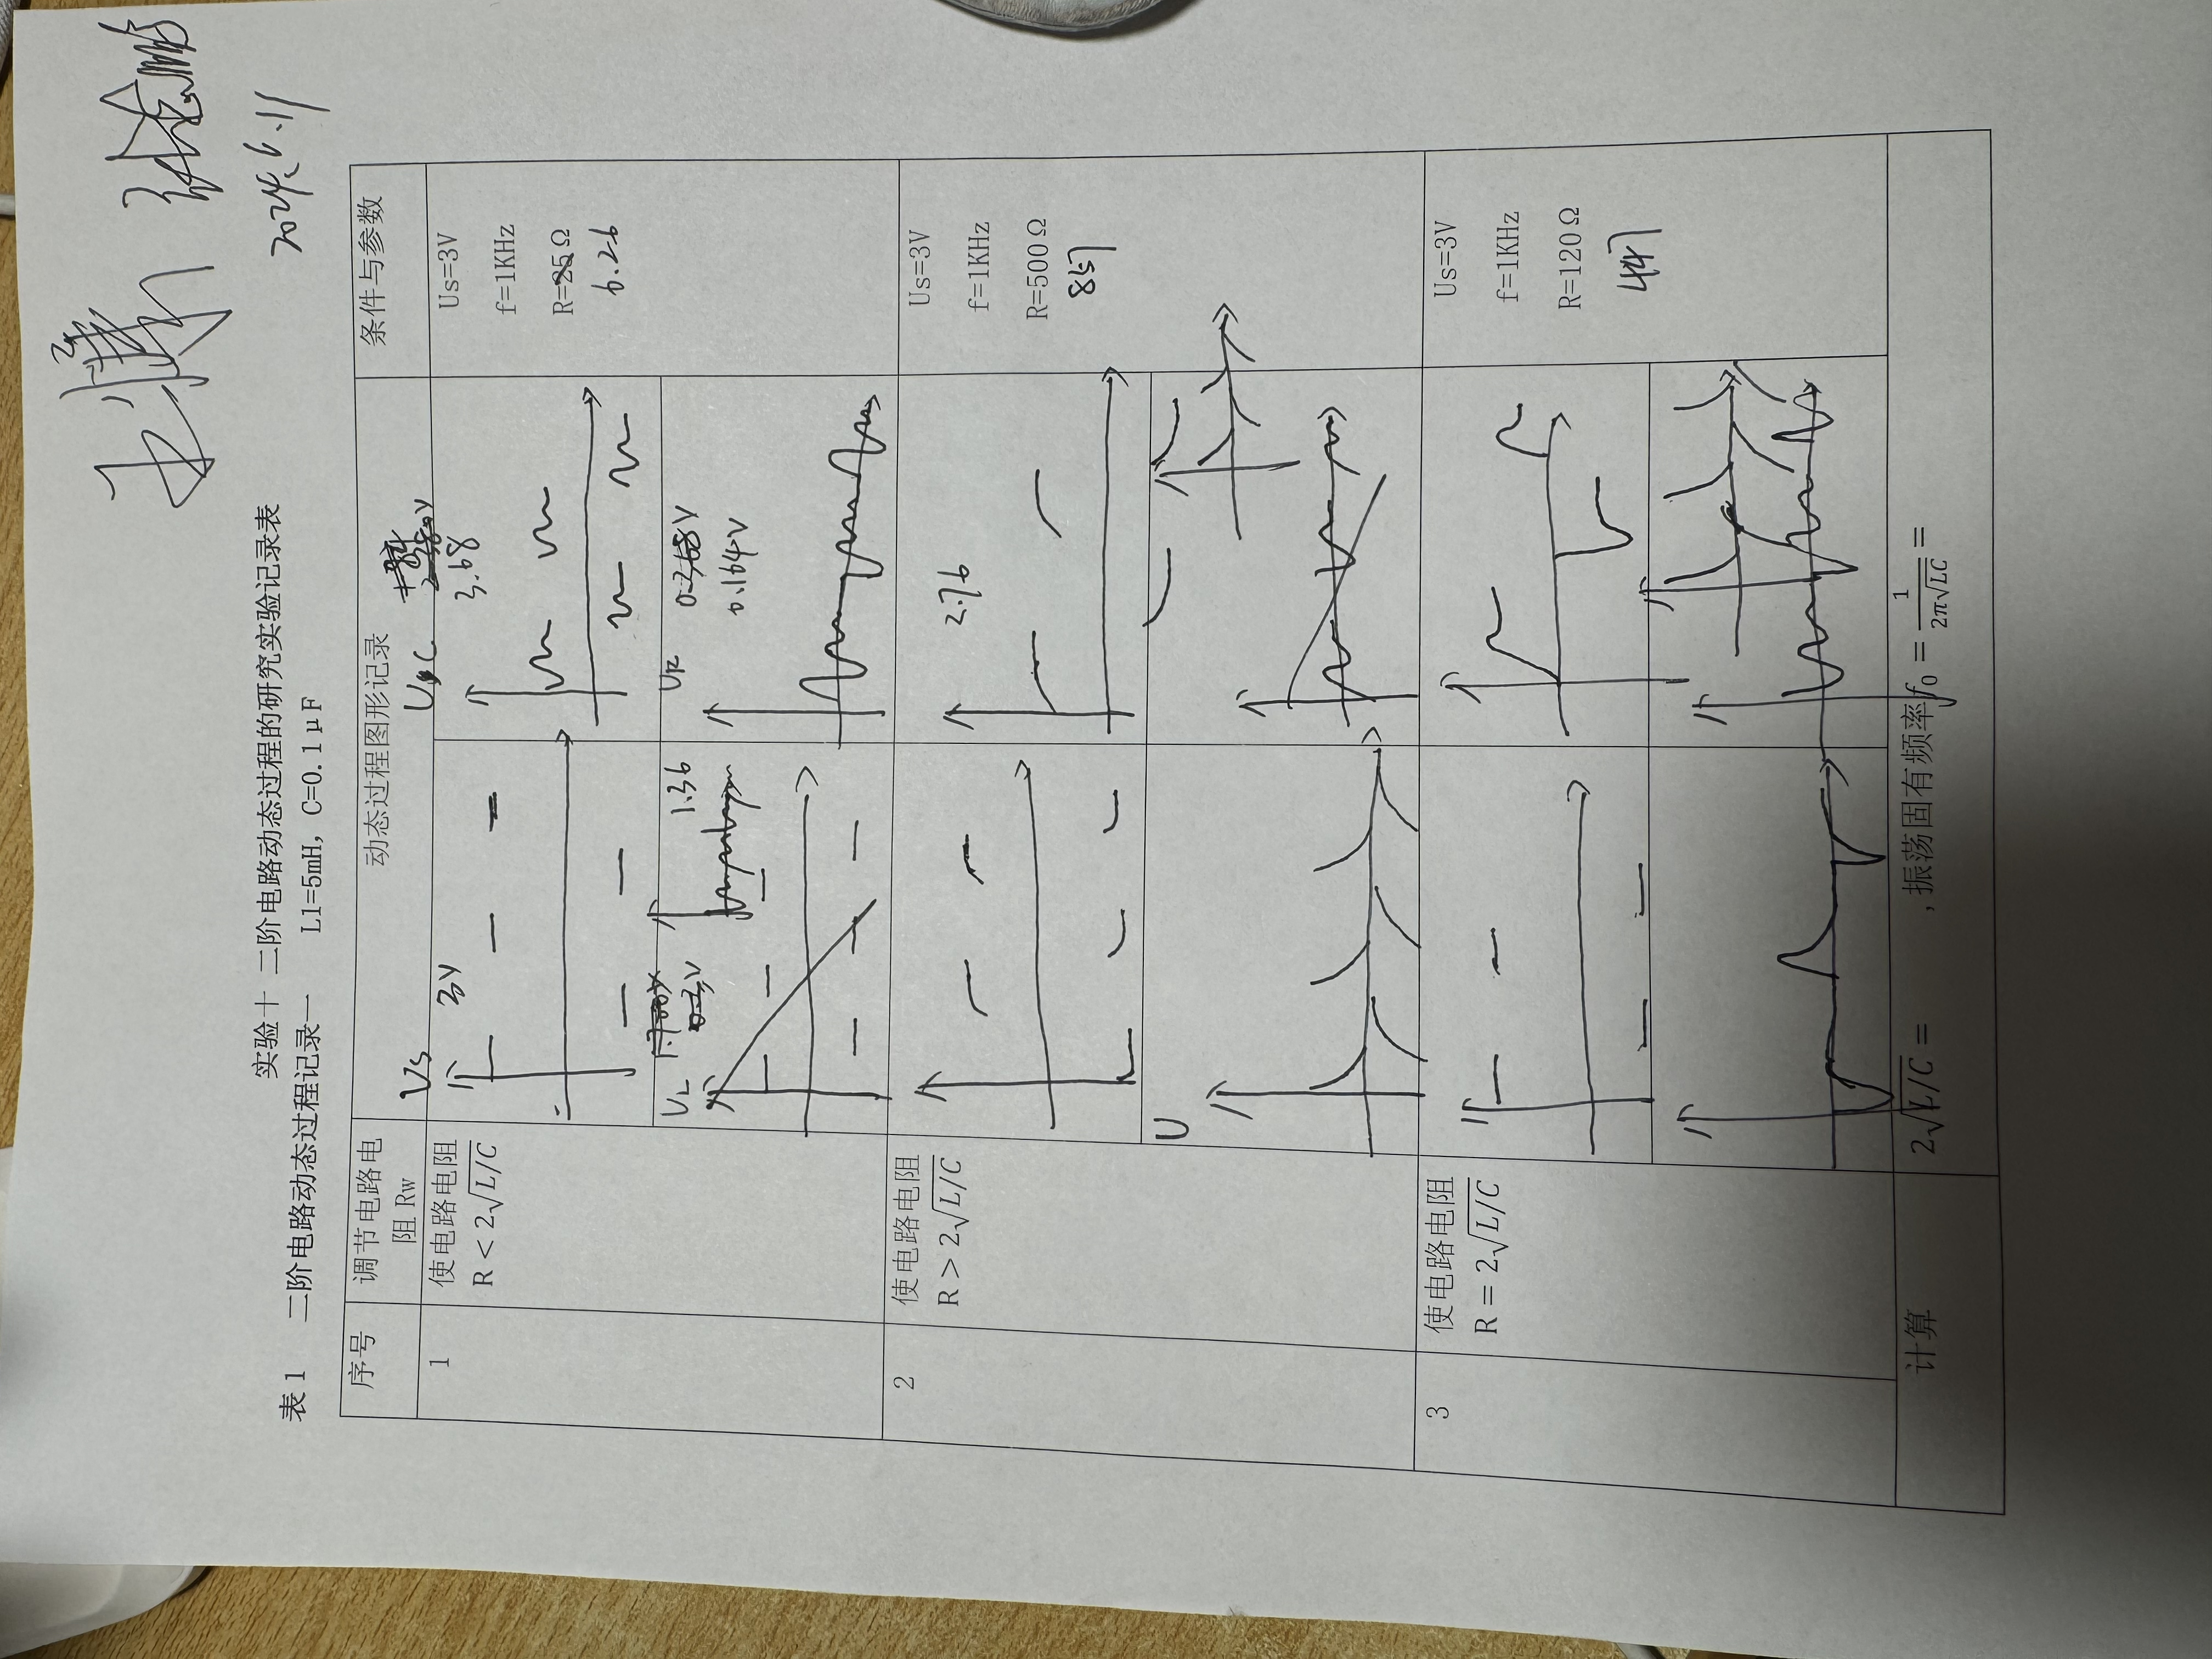
\includegraphics[width=0.95\textwidth]{rawdata.jpg}
\end{figure}
\end{document}